%#!platex main

\chapter{目的プログラム生成}

本講義の最後として、目的プログラムの生成について述べる。ただし、C言語の構
文すべてを扱うと内容が複雑になるので、ここでは概略を述べるにとどめる。ま
た\ref{083441_12Apr06}章に引き続き、具体性を持たせるために、Pentium プロ
セッサのAT\&T形式アセンブリ言語を目的言語とするが、本章で述べる内容は汎用
的なものである。

% 構文主導定義による中間コード生成の概略。アセンブリ言語生成の例。

まず初めに、C言語の代表的な文について、どのような機械語コードを生成すれば
いいのか述べる。次に、そのいくつかについて、解析木からコードを生成する方
法について検討する。

\section{C言語の文に対する機械語コード}

\subsection{複文}

C言語の複文は次のような形式である。
\begin{quote}
 \icode{\{ $宣言文_1$; $\cdots$ $宣言文_n$; $文_1$; $\cdots$ $文_m$; \}}
\end{quote}
「宣言文」とは変数の宣言、「文」とは宣言文以外のC言語の文である。C言語で
は、複文の先頭に変数の宣言を置くことができ、複文内で宣言された変数は、そ
の複文内でのみ有効な局所変数となる。

これに対応する機械語コードは、次のような構造になる。
\begin{quote}
 $宣言文_1, \cdots, 宣言文_n$に対応する変数領域の確保\\
 $宣言文_1$の初期化(もしあれば) \\
 $\cdots$ \\
 $宣言文_n$の初期化(もしあれば) \\
 $文_1$の実行 \\
 $\cdots$ \\
 $文_m$の実行 \\
 局所変数領域の解放
\end{quote}
局所変数領域の確保は、具体的には、実行時スタック上に局所変数分の領域を
(\icode{push}命令などで)積むことに相当する。ただし、変数の初期化や$文_1,
\cdots, 文_m$で変数の参照が起こるため、それぞれの局所変数の領域がどこに確
保されたのか、複文のコード生成中、記憶しておく必要がある。これは通常、確
保された領域の番地を記号表に書き込むことで対処する。例えば、
\begin{quote}
 \icode{int x = 10;}
\end{quote}
という宣言文に対して\icode{x}の領域を実行時スタック上に(例えば
\icode{-16(\%ebp)}に)確保するとすると、\icode{-16(\%ebp)}を記号表の
\icode{x}の項目に書き込む。次いでこの初期化として、次のような機械語を生成
する。
\begin{quote}
\begin{lstlisting}[language={[x86masm]Assembler}]
 movl  -16(%ebp), 10
\end{lstlisting}
\end{quote}

複文の中で確保した局所変数領域は、複文終了時に(\icode{pop}命令などで)実行
時スタックから下ろすようにする。

\subsection{条件文}

C言語の条件文の典型的な形は次のようになる。
\begin{quote}
 \icode{if ({\rm 条件式}) $文_1$ else $文_2$}
\end{quote}
これに対応する機械語コードは次のようになる。
\begin{quote}
 \begin{tabular}{ll}
  & 条件式を計算し、結果をレジスタ$R$に格納 \\
  & \icode{cmpl $R$, 0} \\
  & \icode{je $L_1$} \\
  & $文_1$の実行\\
  & \icode{jmp $L_2$}\\
  $L_1$: & $文_2$の実行 \\
  $L_2$: & \\
 \end{tabular}
\end{quote}
C言語では、条件式が0以外なら真($文_1$が実行)、0なら偽($文_2$が実行)と
見なされることに注意されたい。

\subsection{繰り返し文}

ここでは繰り返し文のうち while 文のみを取り上げる。while文の形式は次のよ
うになる。
\begin{quote}
 \icode{while ({\rm 条件式}) {\rm 文}}
\end{quote}
これに対する機械語コードは次のようになる。
\begin{quote}
\begin{tabular}{ll}
 $L_1$: & 条件式を計算し、結果をレジスタ$R$に格納 \\
        & \icode{cmpl $R$, 0} \\
        & \icode{je $L_2$} \\
        & \icode{jmp $L_1$} \\
 $L_2$: & \\
\end{tabular}
\end{quote}
もしwhile文の中に\icode{break}文があれば、(while文から脱出するということ
であるから)\icode{jmp $L_2$}を挿入すればよい。また\icode{continue}文があ
れば(次の繰り返しに進むということであるから)\icode{jmp $L_1$}を挿入すれば
よい。

\subsection{式文}

式文は、C言語の代入文や関数呼び出しの総称である\footnote{正確には、式$e$
を実行するだけの文である。$e$に変数への代入が含まれる場合には、副作用によっ
て変数に計算結果の値が残るとみなされる。プログラム実行の副作用については
「計算機言語I」の講義内容を参照のこと。}。関数呼び出しがどのようなコード
になるかは\ref{181902_17Apr06}節で述べたので、ここでは代入文について取り
上げる。

変数\icode{v}への代入文\icode{v = $e'$;}に対する機械語コードは次のように
なる。ただし$loc(v)$は、変数\icode{v}が割り当てられている番地を表す。
\begin{quote}
 $e'$の計算を行い、結果をレジスタ$R$に格納 \\
 \icode{movl $R$, $loc(v)$}
\end{quote}

したがって、\icode{i = foo();}のように$e'$が関数呼び出しの場合には、次の
ようなコードが生成される。関数からの返り値はレジスタ\icode{\%eax}に格納さ
れることを思い出しておくこと。
\begin{quote}
 \icode{call \_foo} \\
 \icode{movl \%eax, $loc(i)$}
\end{quote}

$e'$が算術式の場合、基本的なコード生成の手順は次のようになる。二項算術演
算子$\circ$に対応して、機械語の算術命令$inst$が用意されているならば、算
術式$e_1 \circ e_2$のための機械語コードは次のようになる。
\begin{quote}
 $e_1$の値をレジスタ$R$にロード \\
 \icode{$inst$ $e_2$の値, $R$}
\end{quote}
例えば式$x+y$に対しては次のようなコードが生成される。
\begin{quote}
 \icode{movl $loc(x)$, $R$} \\
 \icode{addl $loc(y)$, $R$}
\end{quote}
また式$a*b+y$に対しては次のようなコードが生成される。
\begin{quote}
 \icode{movl $loc(a)$, $R$} \\
 \icode{imul $loc(b)$, $R$} \\
 \icode{movl $R$, $R'$} \\
 \icode{addl $loc(y)$, $R'$}
\end{quote}
$a*b$の計算結果はレジスタ$R$に残っているので、3行目ではレジスタ$R$の値を
レジスタ$R'$にロードする、というコードを生成している。

\subsection{コード生成の問題}

ここまでの節で述べてきた機械語コードは原則的なもので、実際はさらに工夫を
行う必要がある。特に、レジスタの割り当てと無駄なコードの除去は充分注意し
なければならない。

例として、上で挙げた式$a*b+y$に対する次のコードを考える。
\begin{quote}
 \icode{movl $loc(a)$, $R$} \\
 \icode{imul $loc(b)$, $R$} \\
 \icode{movl $R$, $R'$} \\
 \icode{addl $loc(y)$, $R'$}
\end{quote}
このコードでは、$a*b$の計算結果をレジスタ$R$に、最終結果をレジスタ$R'$に
それぞれ割り当てている。しかし、この例では最終結果も$R$に割り当てても構わ
ないはずである。すると次のようなコードになり、3つの機械語命令で済み、また
使用するレジスタも1つで済む。
\begin{quote}
 \icode{movl $loc(a)$, $R$} \\
 \icode{imul $loc(b)$, $R$} \\
 \icode{addl $loc(y)$, $R$}
\end{quote}

汎用レジスタの個数は少ないので、無駄なく汎用レジスタを使い回すことは、速
いコードを生み出すのに大変重要である。

また機械語命令の数を減らすことも重要である。「たかが機械語命令1つ減らした
ところで、大して速くなるわけではない」と思うかもしれないが、これが100万回
のループの中のコードだったらどうだろう。40秒かかった計算が30秒で済むかも
しれない。

いったん生成したコードを変形し、より速く効率よいコードに改良することを
{\bfseries 最適化}(optimization)という。本講義ではこれ以上深入りしない
が、最適化を行うには、解析木からいきなり目的プログラムの機械語命令を生成
するのではなく、次節で述べるように、中間的な形式のコード(中間コード)を
生成するほうがよい。最適化のためのコード解析が、機械語命令に対してよりも
中間コードに対するほうが行いやすいからである。

\section{翻訳スキームに基づくコード生成}

この節では、翻訳スキームに基づいて解析木から中間コードを生成する方法につ
いて述べる。ただし、簡単のため、取り上げるのは算術式とwhile文にとどめる。

\subsection{三番地コード}

ここでは中間コードとして{\bfseries 三番地コード}(three-address code)と
いうものを用いる。三番地コードの文のうち、本節の説明に必要なものを以下に
示す。なお、三番地コードの全命令は\cite{aho86:_compiler}の8.1節にある。

\begin{enumerate}
 \item 代入文\icode{x = y $\op$ z}。ここで$\op$は二項算術演算子である。
 \item 代入文\icode{x = $\op$ y}。ここで$\op$は単項演算子(符号の反転を表す
       $-$など)である。
 \item 代入文\icode{x = y}。$y$の値を$x$に代入する。
 \item 無条件分岐\icode{goto $L$}。$L$をラベルに持つ文に分岐する。
 \item 条件付き分岐\icode{if x $\op$ y goto $L$}。$\op$は比較演算子である。
       \icode{x $\op$ y}が成立すれば$L$をラベルに持つ文に分岐する。成立し
       なければ次の文に制御を移す。
\end{enumerate}

これらから分かるように、三番地コードでは、文の右辺には演算子をたかだか1
つしか許さない。2つ以上演算子を含む算術式については、一時変数を用いて、複
数の文の列に翻訳しなければならない。たとえば$x + y * z$という原始言語の式
は、次のような文の列になる。
\begin{quote}
 \icode{t1 = y * z} \\
 \icode{t2 = x + t1}
\end{quote}

\subsection{三番地コードを生成する翻訳スキーム}

多くの場合、三番地コードは\ref{195223_17Apr06}節で述べたS属性定義やL属性
定義を用いて、解析木から生成することができる。

まず、右辺に算術式を持つ代入文を考えよう。生成規則は次のようになる。
\begin{align*}
 S & \rightarrow \icode{id} = E \\
 E & \rightarrow E + E \\
 E & \rightarrow E \ast E \\
 E & \rightarrow - E \\
 E & \rightarrow ( E ) \\
 E & \rightarrow \icode{id}
\end{align*}
\begin{figure}
 \begin{center}
  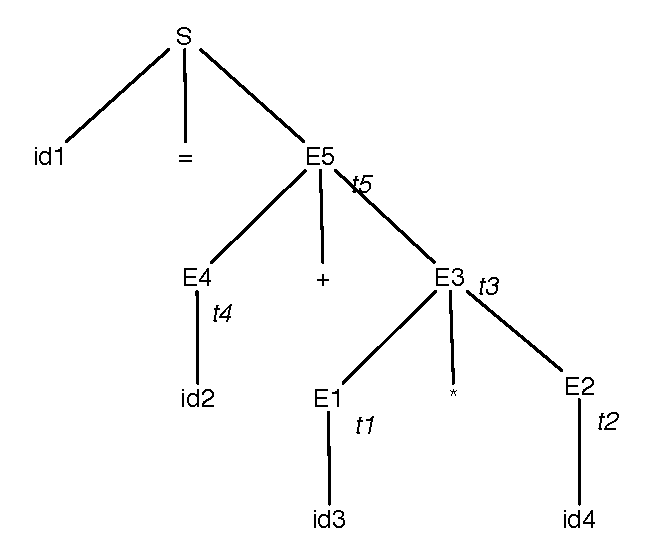
\includegraphics{figure/parse_tree_substitution.pdf}
 \end{center}
 \caption{代入文\icode{id = id + id * id}に対する解析木}
 \label{142215_18Apr06}
\end{figure}
この文法に基づき、代入文\icode{id = id + id * id}の解析木を作ると図
\ref{142215_18Apr06}のようになる。

この代入文に対する三番地コードには、さまざまな可能性がある。ここでは、解
析木中の内部節点(非終端記号)$E$それぞれに一時変数を割り振るものとしよう
(図\ref{142215_18Apr06}中の斜字体)。すると、対応する三番地コードは次の
ようになる\footnote{明らかに冗長な文が含まれているが、これは最適化によっ
て改善するものとし、ここでは問題にしない。}。コード中、関数$val(id)$は識
別子$id$の値を表す。
\begin{align*}
 t_4 & = val(id_2) && E_4 \\
 t_1 & = val(id_3) && E_1 \\
 t_2 & = val(id_4) && E_2 \\
 t_3 & = t_1 \ast t_2 && E_3 \\
 t_5 & = t_4 + t_3 && E_5 \\
 id_1 & = t_5 && S
\end{align*}

明らかに各文はそれぞれ右に示した内部節点に対応しており、かつその節点の子
節点の一時変数のみに依存している。しかも、対応する内部節点の出現順は、解
析木を帰りがけ順にたどった順に一致している。

したがって、上記の三番地コードはS属性定義によって生成することが可能である。
以下に三番地コードを生成するS属性定義を示す。ここで、非終端記号の属性
$place$は、その非終端記号に対応する一時変数名を保持している。また関数
$newtemp()$は新たな一時変数を生成する関数、$gencode()$は引数から三番地コー
ドを生成する関数である。
\begin{align*}
 S \rightarrow & \icode{id} = E\ \{ gencode(\icode{id = } E.place);\} \\
 E \rightarrow & \{E.place = newtemp(); \} \\
   & E_1 + E_2\ \{ gencode(E.place = E_1.place + E_2.place); \}\\
 E \rightarrow & \{E.place = newtemp(); \} \\
   & E_1 \ast E_2\ \{ gencode(E.place = E_1.place * E_2.place); \} \\
 E \rightarrow & \{E.place = newtemp(); \} \\
   & - E_1\ \{ gencode(E.place = - E_1.place); \}\\
 E \rightarrow & \{E.place = newtemp(); \} \\
   & ( E_1 )\ \{ gencode(E.place = E_1.place); \} \\
 E \rightarrow & \{E.place = newtemp(); \} \\
   & \icode{id}\ \{ gencode(E.place = val(\icode{id})); \}
\end{align*}

もう一つ、翻訳スキームを用いた三番地コード生成の例として、while文を取り上
げる。while文の生成規則は次のようになる。
\begin{align*}
 S & \rightarrow \icode{while}\ (E)\ S
\end{align*}
これに対応する三番地コードは次のようになる。添字の$r$は右辺に出現する記号
であることを表す。
\begin{quote}
 \begin{tabular}{ll}
  $L_1$: & $E$に対するコード \\
        & \icode{if $E.place$ = 0 goto $L_2$} \\
        & $S_r$に対するコード \\
        & \icode{goto $L_1$} \\
  $L_2$: & \\
 \end{tabular}
\end{quote}

これも代入文と同様、S属性定義を用いて解析木から生成することが可能である。
以下にこの三番地コードを生成するS属性定義を示す。ここで属性$begin, end$
はそれぞれ$L_1, L_2$に相当するラベルを保持する。また関数$newlabel()$は、
新たなラベルを生成する関数である。
\begin{align*}
 S \rightarrow & \{ S.begin = newlabel();\ S.end = newlabel(); \} \\
               & \{ gencode(S.begin\colon); \} \\
               & \icode{while}\ (E)\ \{ /*ここまででEのコードが生成され
 ている */\} \\
               & \{ gencode(\icode{if}\ E.place = 0\ \icode{goto}\ S.end);
 \} \\
               & S\ \{ /*ここまででS_rのコードが生成されている */\} \\
               & \{ gencode(\icode{goto}\ S.begin); \} \\
               & \{ gencode(S.end\colon); \} 
\end{align*}
